\documentclass[10pt, a4paper]{article}
\usepackage[utf8]{inputenc}
\usepackage{amsmath, amssymb}
\usepackage{graphicx}
\usepackage{float}
\usepackage{tikz}
\usetikzlibrary{shapes.geometric, arrows.meta, positioning, fit}
\usepackage{geometry}
\geometry{margin=1in}
\usepackage{booktabs}
\usepackage{hyperref}

\title{\textbf{6G Cognitive-Hierarchical Swarm Routing (CHSR) Optimization under Dynamic Blockages}}
\author{Simulation Report}
\date{\today}

\begin{document}
\maketitle

\section{Introduction}
The Terahertz (THz) band (e.g., 300 GHz) provides extreme data rates for 6G networks but suffers from severe propagation losses and susceptibility to physical blockages. This report details the formulations, computational complexity, and performance of a Cognitive-Hierarchical Swarm Routing (CHSR) system driven by Adaptive Particle Swarm Optimization (APSO).

\section{System Model and Formulations}
\subsection{3D Propagation and Attenuation}
The spatial domain is discretized into a 2D floor plan of $32 \times 20$ meters with a ceiling height of $3.0$ m. The Signal-to-Interference-plus-Noise Ratio (SINR) for a user $u$ at coordinates $(x_u, y_u, z_u)$ served by router $r$ at $(x_r, y_r, z_r)$ is determined by the received power $P_{\text{rx}}$.

The base Free-Space Path Loss (FSPL) and molecular absorption are given by:
\begin{equation}
    P_{\text{FSPL}} = 20 \log_{10} \left( \frac{4 \pi f d_{3D}}{c} \right), \quad P_{\text{abs}} = 4.343 \cdot k(f) \cdot d_{3D}
\end{equation}
where $d_{3D}$ is the volumetric Euclidean distance, $f=300$ GHz, and $k(f)$ is the molecular absorption coefficient.

\subsection{Static Infrastructure Blockage Model}
The environment contains custom static walls (solid concrete, wood, glass). A parametric line equation is drawn from the router to the user. The spatial line intersects horizontal ($y=y_w$) and vertical ($x=x_w$) walls. The static loss $L_{\text{static}}$ is the summation of material-specific penalties $M_w$:
\begin{equation}
    L_{\text{static}} = \sum_{w \in W_{\text{intersect}}} M_w \cdot \mathbb{I}(z_i \leq h_w)
\end{equation}
where $z_i$ is the height of the signal beam at the point of intersection, and $h_w$ is the physical height of the wall. 

\subsection{Dynamic Human Crowd Density}
Human mobility is modeled as a time-varying probability density matrix $D_h(x,y,t)$. The human blockage penalty $L_{\text{dynamic}}$ is integrated along the 2D projection of the signal path. If the beam elevation $z(c)$ drops below the human height $H_h$ at grid cell $c$, the expected penalty is applied:
\begin{equation}
    L_{\text{dynamic}} = \sum_{c \in \text{Path}} D_h(c, t) \cdot P_{\text{human}} \cdot \mathbb{I}(z(c) \leq H_h)
\end{equation}
where $P_{\text{human}} = 20$ dB.

\section{Hierarchical APSO Workflow}
To minimize mechanical actuation latency, the APSO algorithm operates hierarchically. The fitness function $F(S)$ maximizes coverage proportion $\Phi$, triggering higher tiers only if $\Phi < 0.85$:
\begin{itemize}
    \item \textbf{Tier 1 \& 2}: Electronic tuning of beamwidth $\alpha$ and azimuth orientation $\phi$.
    \item \textbf{Tier 3}: Vertical translation $z$ adjustments.
    \item \textbf{Tier 4}: Full spatial translation $x, y$ adjustments.
\end{itemize}

During active optimization, the APSO velocity ($v_i$) and position ($x_i$) vector updates for the $i$-th particle at iteration $k$ are evaluated continuously across the permitted tier dimensions:
\begin{align}
    v_i^{k+1} &= w \cdot v_i^k + c_1 r_1 (p_{\text{best},i} - x_i^k) + c_2 r_2 (g_{\text{best}} - x_i^k) \\
    x_i^{k+1} &= x_i^k + v_i^{k+1}
\end{align}
where $w = 0.9 - 0.5 (k / K_{\max})$ acts as a linearly decaying adaptive inertia weight, $c_1, c_2$ are cognitive and social coefficients (set to 1.5), and $r_1, r_2 \sim \mathcal{U}(0, 1)$ are random stochastic variables. The vector $p_{\text{best},i}$ represents the particle's historical best state, while $g_{\text{best}}$ designates the global optimum discovered by the swarm.

\begin{figure}[H]
    \centering
    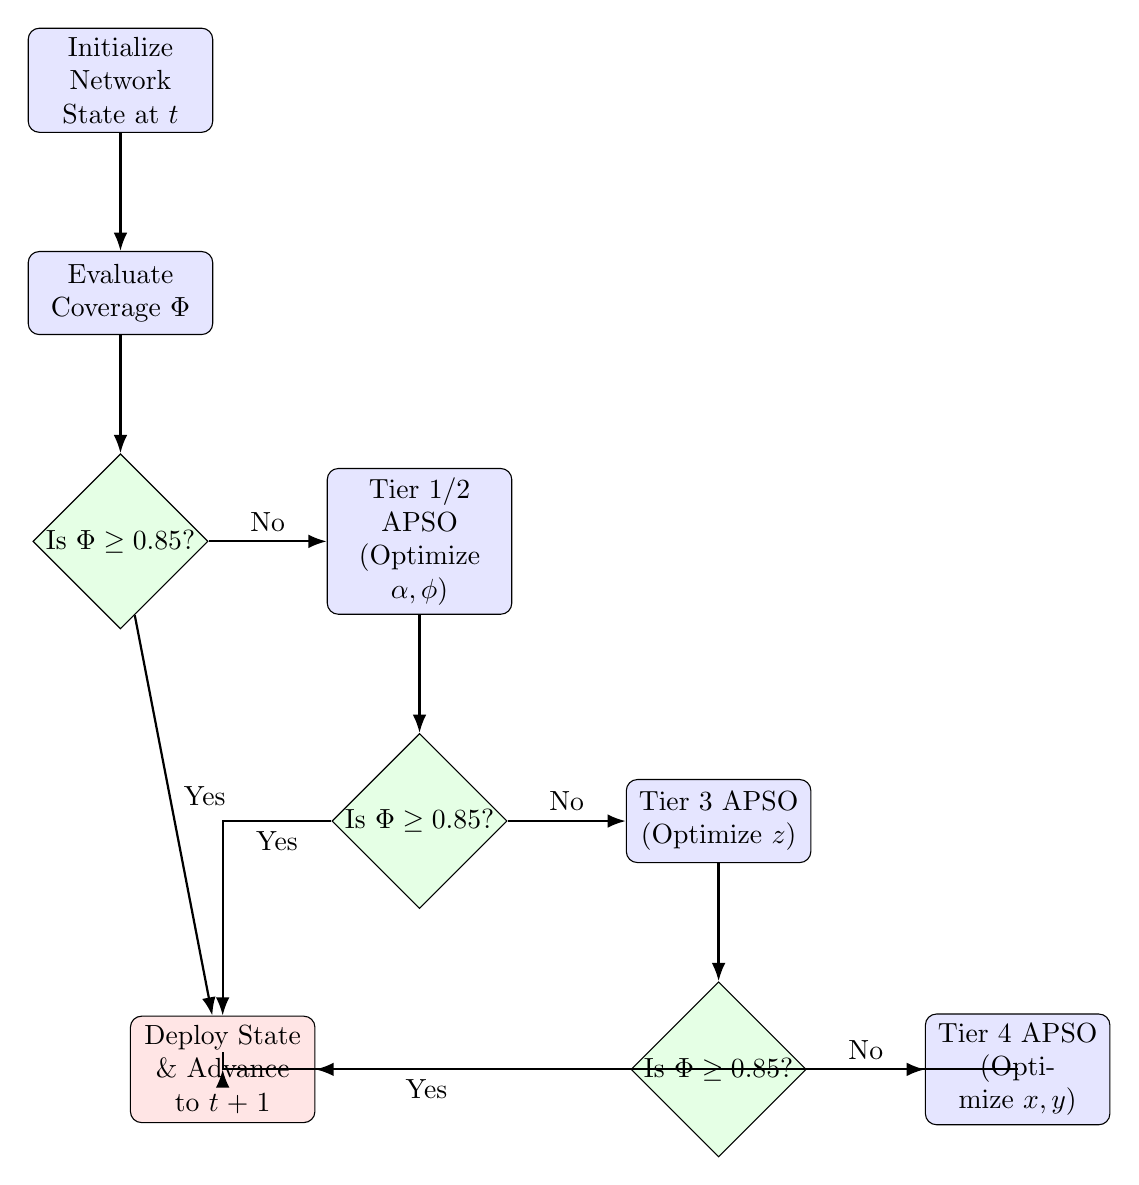
\begin{tikzpicture}[node distance=1.5cm, auto, 
        block/.style={rectangle, draw, fill=blue!10, text width=6em, text centered, rounded corners, minimum height=3em},
        decision/.style={diamond, draw, fill=green!10, text width=5.5em, text badly centered, inner sep=0pt},
        line/.style={draw, -Latex, thick}]
        
        \node [block] (init) {Initialize Network State at $t$};
        \node [block, below=of init] (eval) {Evaluate Coverage $\Phi$};
        \node [decision, below=of eval] (check) {Is $\Phi \geq 0.85$?};
        \node [block, right=1.5cm of check] (t1) {Tier 1/2 APSO (Optimize $\alpha, \phi$)};
        \node [decision, below=of t1] (check2) {Is $\Phi \geq 0.85$?};
        \node [block, right=1.5cm of check2] (t3) {Tier 3 APSO (Optimize $z$)};
        \node [decision, below=of t3] (check3) {Is $\Phi \geq 0.85$?};
        \node [block, right=1.5cm of check3] (t4) {Tier 4 APSO (Optimize $x, y$)};
        \node [block, left=4cm of check3, fill=red!10] (done) {Deploy State \& Advance to $t+1$};
        
        \path [line] (init) -- (eval);
        \path [line] (eval) -- (check);
        \path [line] (check) -- node {Yes} (done);
        \path [line] (check) -- node {No} (t1);
        \path [line] (t1) -- (check2);
        \path [line] (check2) -| node[pos=0.25] {Yes} (done);
        \path [line] (check2) -- node {No} (t3);
        \path [line] (t3) -- (check3);
        \path [line] (check3) -| node[pos=0.25] {Yes} (done);
        \path [line] (check3) -- node {No} (t4);
        \path [line] (t4) |- (done);
        
    \end{tikzpicture}
    \caption{Hierarchical APSO Workflow}
\end{figure}

\section{Time Complexity Analysis}
The time complexity of the algorithm is dominated by the ray-tracing required to evaluate the SINR map for the APSO fitness function.
Let $N$ be the number of APs, $L \times B$ be the grid dimensions, $P$ be the number of APSO particles, and $I$ be the number of iterations.
\begin{itemize}
    \item \textbf{Ray Tracing \& Path Loss Calculation}: For a single router to all grid cells, determining static wall intersections and human density traversals takes $\mathcal{O}(L \cdot B \cdot \max(L, B) \cdot W)$, where $W$ is the number of walls.
    \item \textbf{SINR Evaluation}: Aggregating $N$ routers takes $\mathcal{O}(N \cdot L \cdot B \cdot \max(L, B) \cdot W)$.
    \item \textbf{APSO Execution}: Evaluating $P$ particles over $I$ iterations takes $\mathcal{O}(P \cdot I \cdot N \cdot L^2 \cdot B \cdot W)$ assuming $L \approx B$.
\end{itemize}
Overall worst-case time complexity per time step (if Tier 4 is reached) is $\mathcal{O}(P \cdot I \cdot N \cdot L^2 \cdot B \cdot W)$. The hierarchical approach drastically reduces the empirical runtime by terminating early at Tier 1/2 whenever possible.

\section{Simulation Parameters}
\begin{table}[H]
    \centering
    \begin{tabular}{@{}ll@{}}
    \toprule
    \textbf{Parameter} & \textbf{Value} \\ \midrule
    Environment Dimensions & $32\text{ m} \times 20\text{ m} \times 3\text{ m}$ \\
    Operating Frequency ($f$) & 300 GHz \\
    Transmit Power ($P_{\text{tx}}$) & 20 dBm \\
    Main-Lobe Gain ($G_{\text{max}}$) & 30 dBi \\
    Beamwidths ($\alpha$) & $30^\circ, 45^\circ, 60^\circ, 75^\circ, 90^\circ, 120^\circ$ \\
    Candidate Z-axis & 2.0 m to 3.0 m (0.2 m step) \\
    Azimuth Increments & $45^\circ$ ($\pi/4$ rad) \\
    Solid/Wood/Glass Penalties & 30 dB / 20 dB / 15 dB \\
    System Noise Floor ($N_0$) & $-94$ dBm \\
    Human Blocker Penalty & 20 dB (Height 1.6 m) \\ \bottomrule
    \end{tabular}
    \caption{System Simulation Parameters}
\end{table}

\section{Results \& Visualizations}
The simulation evaluated the custom spatial constraints against shifting human blockages.
\begin{figure}[H]
    \centering
    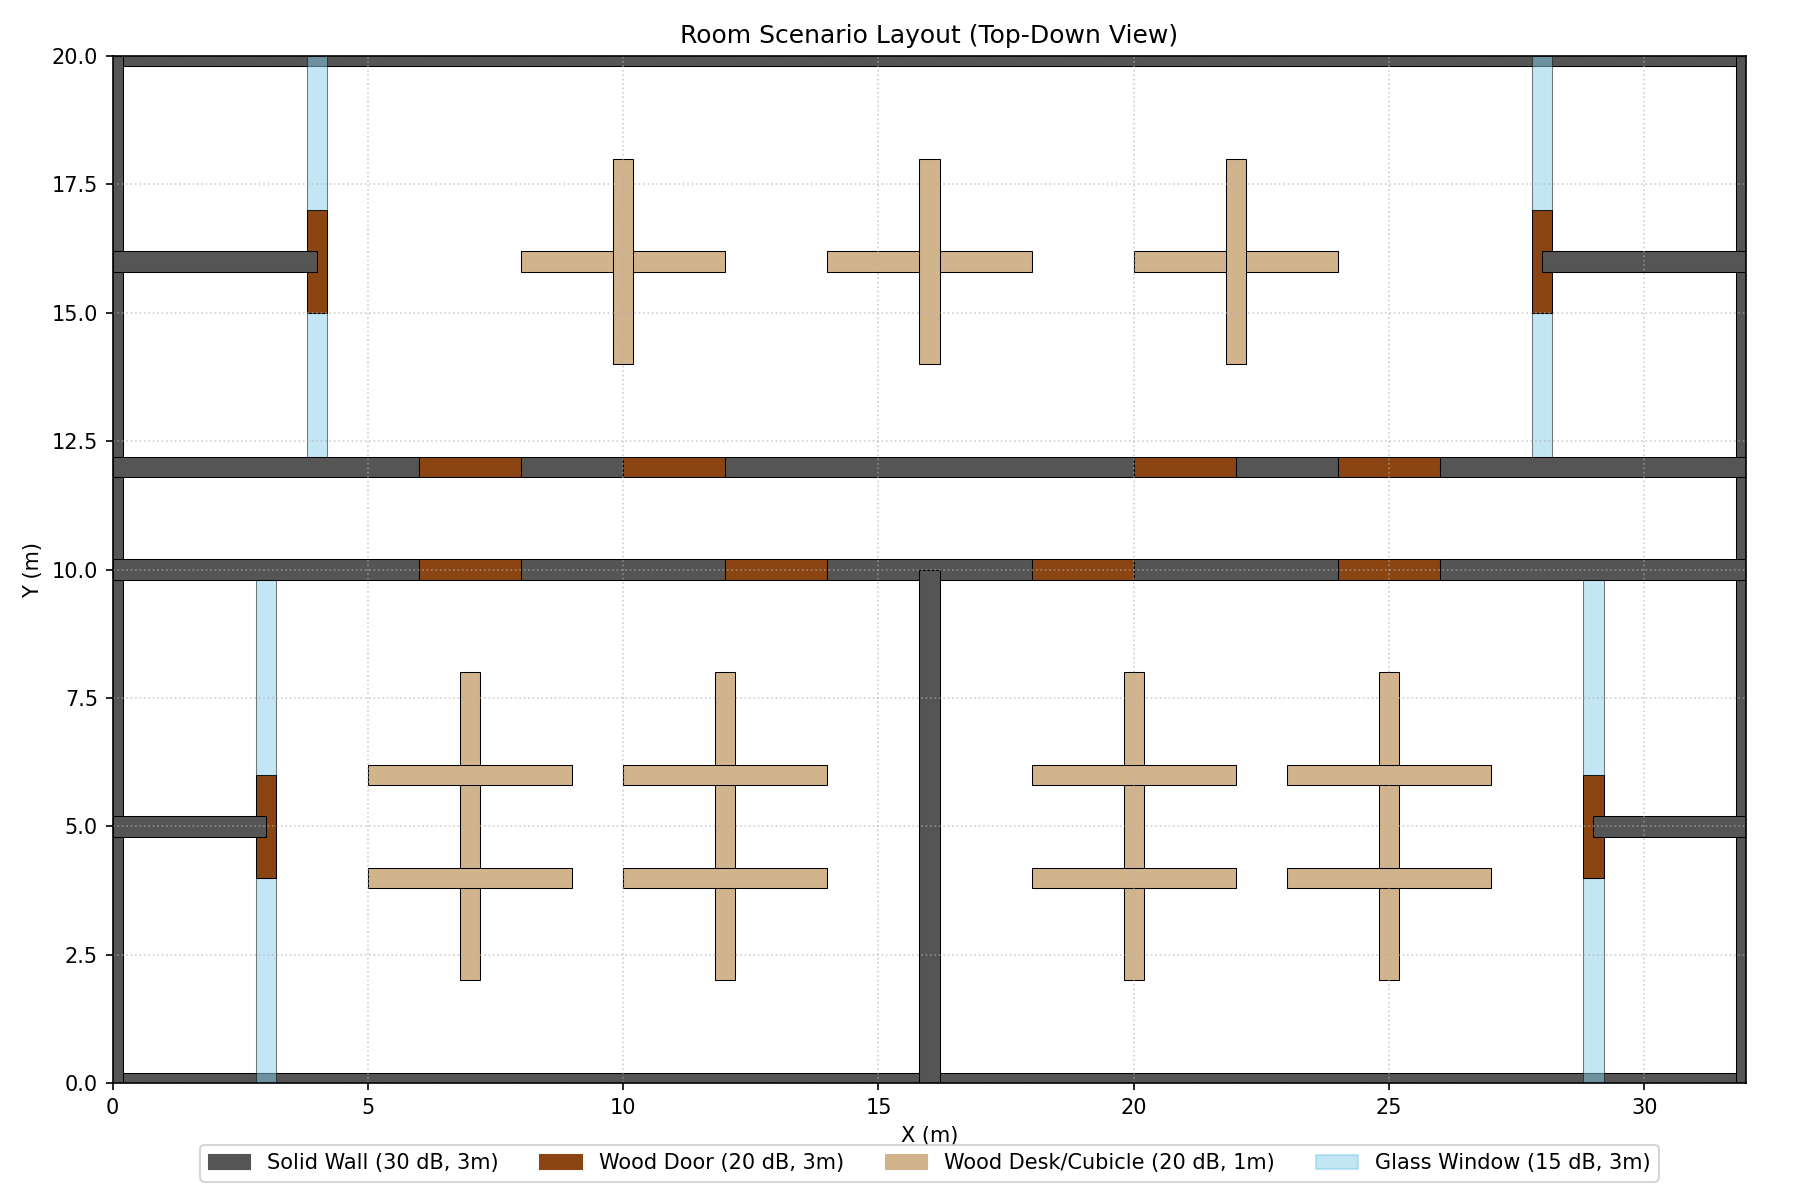
\includegraphics[width=0.8\textwidth]{room_scenario.png}
    \caption{Modeled Room Infrastructure Layout.}
\end{figure}

\begin{figure}[H]
    \centering
    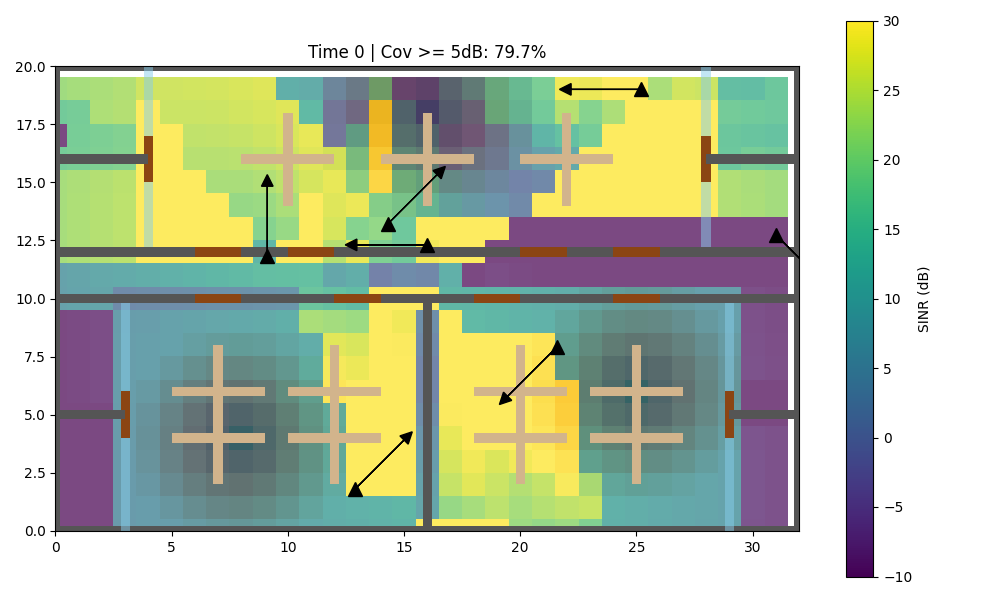
\includegraphics[width=0.48\textwidth]{simulation_t0.png}
    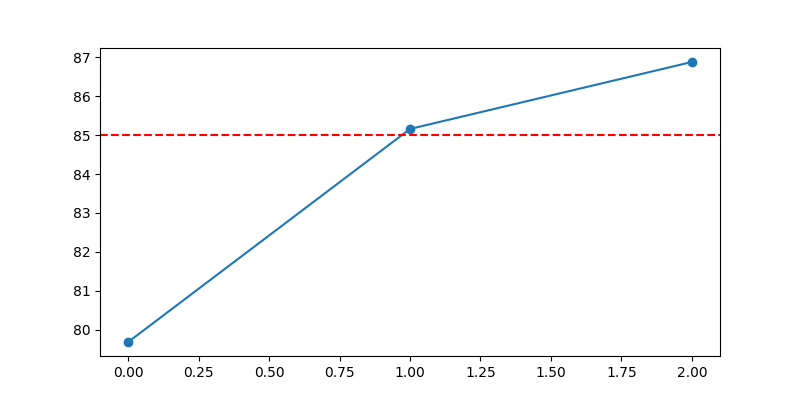
\includegraphics[width=0.48\textwidth]{coverage_over_time.png}
    \caption{Left: Spatial SINR Heatmap Post-APSO Tier 4 Optimization ($t=0$). Right: Sustained Coverage Threshold over Time.}
\end{figure}

\end{document}
